%%%%%%%%%%%%%%%%%%%%%%%%%%%%%%%%%%%%%%%%%%%%%%%%%%%%%%%%%%%%%%%%%%%%%%
%%                     Process
%%%%%%%%%%%%%%%%%%%%%%%%%%%%%%%%%%%%%%%%%%%%%%%%%%%%%%%%%%%%%%%%%%%%%%

\subsection{Glyph: \glyph{Process}}
\label{sec:process}

A process is the basic process node in SBGN.  It describes a process that transforms a given set of biochemical entities---macromolecules, simple chemicals or unspecified entities---into another set of biochemical entities.  Such a transformation might imply modification of covalent bonds (conversion), modification of the relative position of constituents (conformational process) or movement from one compartment to another (translocation). A process transforms a set of entity pools (represented by \glyph{EPNs} in \SBGNPDLone) into another set of entity pools. A \glyph{process} is represented by a square box linked to two connectors, small arcs attached to the centers of opposite sides. The consumption (\sect{consumption}) and production (\sect{production}) arcs are linked to the extremities of those connectors. The modulatory arcs (\sect{arcs}) point to the other two sides of the box. A \glyph{process} connected to \glyph{production} arcs on opposite sides is a reversible process. 

\begin{figure}[H]
  \centering
  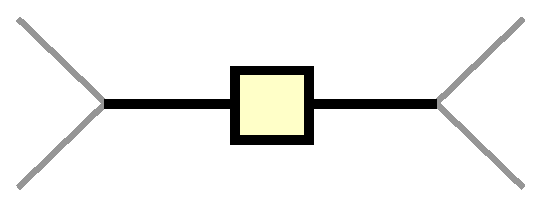
\includegraphics[scale = 0.4]{images/process}
  \caption{The \PD glyph for \glyph{process}.}
  \label{fig:process}
\end{figure}

The example in \fig{trans-react} illustrates the use of a \glyph{process} node to represent a reaction between two reactants that generates three products. The stoichiometry for each entity pool involved is 1, and therefore can be omitted.  

\begin{figure}[H]
  \centering
  \includegraphics[scale = 0.3]{images/process-reaction}
  \caption{Reaction between ATP and fructose-6-phosphate to produce fructose-1,6-biphosphate, ADP and a proton.}
  \label{fig:trans-react}
\end{figure}

The example in \fig{trans-phos} illustrates the use of a \glyph{process} node to represent the phosphorylation of a protein. 

\begin{figure}[H]
  \centering
  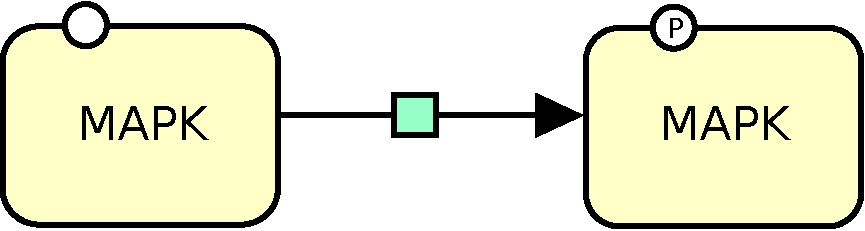
\includegraphics[scale = 0.3]{images/process-phosphorylation}
  \caption{Phosphorylation of the protein MAP kinase.}
  \label{fig:trans-phos}
\end{figure}


The example in \fig{trans-trans} illustrates the use of a \glyph{process} node to represent a translocation. The large round-cornered rectangle represents a compartment border (see \sect{compartment}).

\begin{figure}[H]
  \centering
  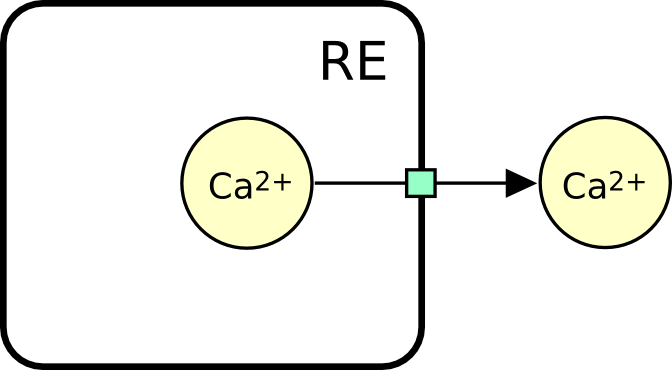
\includegraphics[scale = 0.3]{images/process-translocation}
  \caption{Translocation of calcium ion out of the endoplasmic reticulum. Note that the \glyph{process} does not have to be located on the boundary of the \glyph{compartment}. A \glyph{process} is not attached to any \glyph{compartment}.}
  \label{fig:trans-trans}
\end{figure}

The example in \fig{trans-dim} presents the conversion of two galactoses into a lactose.  Galactoses are represented by only one \glyph{simple chemical}, the cardinality being carried by the \glyph{consumption} arc.

\begin{figure}[H]
  \centering
  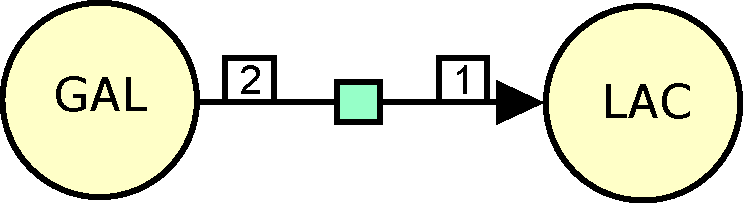
\includegraphics[scale = 0.3]{images/process-dimerisation}
  \caption{Conversion of two galactoses into a lactose.}
  \label{fig:trans-dim}
\end{figure}

